\chapter{Implementation}
\section{Tech Stack Justification}
\import{chapter/05_implementation/backend}{backend_arch.tex}
\section{ Interface and Features}

Our development journey began with a thorough analysis of the client’s requirements to ensure a clear understanding of the project goals and user needs. This foundational step allowed us to identify both functional and non-functional aspects critical to delivering a seamless multilingual virtual tour assistant. Following this, we carefully evaluated and selected the most suitable technologies to meet these requirements efficiently and maintainably. To visualise the user experience and interface, we created detailed wireframes and interactive prototypes using Figma, which facilitated early feedback and iterative improvements before moving into full development.

\subsection{Client Requirements}

\textbf{Note:} We need to decide whether this section will be here or elsewhere and we have not finalized the clear requirements.

\subsection{Tech Stack Selection and Justification}

With a comprehensive understanding of the client's requirements, our next step was to carefully evaluate and select a technology stack that balances scalability, maintainability, performance, and developer experience. Each layer of the frontend architecture was considered through a comparative analysis of available tools and frameworks, ensuring that the final selections aligned with the project’s long-term goals.

\begin{table}[H]
\centering
\caption{Programming Language Comparison}
\begin{tabular}{|l|p{6cm}|p{6cm}|}
\hline
\textbf{Criteria}       & \textbf{JavaScript} & \textbf{TypeScript} \\
\hline
Typing                  & Dynamic             & Static             \\
Ease of Learning        & Easy                & Moderate           \\
Tooling Support        & Excellent           & Excellent          \\
Performance            & Good                & Good               \\
Reason                 & No static typing, harder to maintain large apps & Static typing improves code quality and maintainability \\
\hline
\end{tabular}
\label{tab:programming-language-comparison}
\end{table}

\textbf{Selected:} TypeScript \par
\textbf{Reasoning:} TypeScript was selected due to its static typing capabilities, which enhance code reliability, readability, and maintainability, especially for large-scale applications. Unlike JavaScript, TypeScript helps catch errors at compile time, making development more robust and reducing runtime bugs. It also offers better IDE support, including autocompletion and refactoring, improving developer productivity.

\vspace{2em}

\begin{table}[H]
\centering
\caption{Frontend Framework/Library Comparison}
\begin{tabular}{|l|p{4cm}|p{4cm}|p{4cm}|}
\hline
\textbf{Criteria}       & \textbf{React}                & \textbf{Angular}               & \textbf{Vue.js}               \\
\hline
Architecture            & Component-based               & Full framework                & Progressive framework         \\
Ecosystem Size          & Very Large                   & Large                        & Medium                       \\
Learning Curve          & Moderate                     & Steep                        & Easy                         \\
Performance             & Excellent                    & Excellent                    & Excellent                    \\
Flexibility             & High                         & Low                          & Moderate                     \\
Reason                  & Balance of flexibility and rich ecosystem & Steeper learning curve, more opinionated & Smaller ecosystem, less corporate support \\
\hline
\end{tabular}
\label{tab:frontend-framework-comparison}
\end{table}

\textbf{Selected:} React \par
\textbf{Reasoning:} React offers a balanced trade-off between flexibility and ecosystem maturity. Its component based architecture allows for modular and reusable UI development. Compared to Angular’s steep learning curve and opinionated structure, React provides more freedom in choosing libraries and tools. While Vue.js is simpler, React has broader community support, more enterprise adoption, and better scalability for complex applications.

\vspace{2em}

\begin{table}[H]
\centering
\caption{State Management Comparison}
\begin{tabular}{|l|p{4cm}|p{4cm}|p{4cm}|}
\hline
\textbf{Criteria}       & \textbf{Redux}              & \textbf{Zustand}              & \textbf{Context API}          \\
\hline
Boilerplate             & High                        & Low                          & Low                          \\
Learning Curve          & Steep                       & Easy                         & Easy                         \\
Performance             & Excellent                   & Excellent                    & Good                         \\
Community Support       & Very Large                  & Growing                      & Built-in React               \\
Reason                  & Powerful but verbose and complex & Lightweight, less boilerplate & Not ideal for complex state \\
\hline
\end{tabular}
\label{tab:state-management-comparison}
\end{table}

\textbf{Selected:} Zustand \par
\textbf{Reasoning:} Zustand was chosen for its minimal boilerplate, simple API, and excellent performance. It enables efficient global state management without the complexity of Redux. While Redux is powerful, it requires a steep learning curve and verbose code. Zustand fits well for modern React apps where simplicity and clarity are valued. Context API is great for light use cases but doesn’t scale effectively for complex state logic, making Zustand a better fit.

\vspace{2em}

\begin{table}[H]
\centering
\caption{Styling Solutions Comparison}
\begin{tabular}{|l|p{4cm}|p{4cm}|p{4cm}|}
\hline
\textbf{Criteria}       & \textbf{CSS}               & \textbf{Tailwind CSS}        & \textbf{DaisyUI}             \\
\hline
Approach                & Traditional                & Utility-first                & Component-based              \\
Customizability         & High                       & Medium                      & Low                         \\
Learning Curve          & Easy                       & Moderate                    & Easy                        \\
Development Speed       & Moderate                   & Fast                        & Very Fast                   \\
Reason                  & Difficult to maintain large stylesheets & Rapid styling, consistent design system & Provides prebuilt components on Tailwind \\
\hline
\end{tabular}
\label{tab:styling-solutions-comparison}
\end{table}

\textbf{Selected:} Tailwind CSS + Daisy UI \par
\textbf{Reasoning:} Tailwind CSS was selected for its utility first approach, which accelerates development and enforces consistent styling across components. DaisyUI, built on top of Tailwind, adds ready-to-use, customizable UI components that speed up design implementation. This combination reduces the need to write custom CSS while keeping the UI modern and clean. Traditional CSS is harder to scale and maintain, and DaisyUI complements Tailwind without compromising flexibility.

\vspace{2em}

\begin{table}[H]
\centering
\caption{Prototyping Tools Comparison}
\begin{tabular}{|l|p{4cm}|p{4cm}|p{4cm}|}
\hline
\textbf{Criteria}       & \textbf{Adobe XD}          & \textbf{Sketch}             & \textbf{Figma}               \\
\hline
Platform                & Desktop/Web                & macOS Desktop               & Web-based                   \\
Collaboration           & Limited                   & Limited                    & Excellent                   \\
Ease of Use             & Easy                      & Moderate                   & Easy                        \\
Prototyping Features    & Good                      & Good                       & Excellent                   \\
Reason                  & Less collaborative than Figma & macOS only, less accessible & Cloud-based, real-time collaboration \\
\hline
\end{tabular}
\label{tab:prototyping-tools-comparison}
\end{table}

\textbf{Selected:} Figma \par
\textbf{Reasoning:} Figma was chosen for its cloud-based, real-time collaboration capabilities, making it ideal for distributed teams. Unlike Adobe XD and Sketch, Figma runs entirely in the browser, requires no installation, and works across operating systems. It supports efficient design handoff with developers and includes powerful prototyping tools. Its accessibility, ease of use, and collaborative features make it the most suitable option for modern UI/UX workflows.

\vspace{2em}

\subsection{Design and Prototyping}

Design and prototyping served as a crucial bridge between client expectations and the final product. Utilizing Figma, we developed interactive wireframes and clickable prototypes to facilitate early validation, clear communication and encouraged collaborative feedback. This iterative design process helped us align the UI/UX with the multilingual and accessibility requirements of our target audience, significantly reducing rework during development.

\textbf{Note:} Will be adding more information based on figures that we are planning to add.

\subsection{Implementation}

After finalizing the Figma prototype, the implementation phase commenced and was structured into iterative sprints. Each iteration focused on delivering incremental features, incorporating design feedback, and enhancing both performance and usability. The following sections provide a breakdown of the three main development iterations undertaken.

\subsubsection{Iteration 1:}
The first iteration focused on standing up a clickable skeleton aligned to the Figma user flows. The goal was to deliver a coherent theme, working navigation, language-scoped routing, page shells for all core areas.

\begin{enumerate}
    \item \textbf{Project Setup and Theme Baseline} \\
    Initialised the project with \texttt{Next.js (App Router)}, \texttt{React}, and \texttt{TypeScript} via \texttt{npm}. Established formatting and linting rules to reduce churn. Added \texttt{Tailwind CSS} and defined a global theme (colours, spacing, type scale) applied through \texttt{globals.css}.

    \item \textbf{Routing and Internationalisation} \\
    Introduced a language-scoped route segment \verb|app/[lang]/...|. Persisted the user’s language in \texttt{localStorage} so choices survive refreshes and deep links; URLs remain shareable in the chosen language.

    \item \textbf{Application Structure} \\
    Used App Router with feature folders to separate pages and reusable components.
    \begin{itemize}
        \item \textit{Pages:} \verb|[lang]/cultural-tips|, \verb|essentials|, \verb|language|, \verb|map|, \verb|recommendations|, plus \verb|layout.tsx| and \verb|page.tsx|.
        \item \textit{Components:} \texttt{NavigationBar}, \texttt{LanguageList}, \texttt{ActionButton}, \texttt{MapComponent}, \texttt{SearchBar}, \texttt{InfoAccordion}.
        \item \textit{Support:} \texttt{mockdata/}, \texttt{public/}, \texttt{types/}, \texttt{globals.css}.
    \end{itemize}

    \item \textbf{Reusable Components (v1)} \\
    Prioritised primitives used across pages:
    \begin{itemize}
        \item \textbf{NavigationBar} — top-level navigation mounted in \verb|app/layout.tsx|.
        \item \textbf{LanguageList} — renders supported languages; writes selection to \texttt{localStorage}.
        \item \textbf{ActionButton} — shared CTA styling (``Start'', ``Change language'').
        \item \textbf{MapComponent} — visual placeholder for the map view.
        \item \textbf{SearchBar / InfoAccordion} — early building blocks for dense content.
    \end{itemize}

    \item \textbf{Page Shells Delivered} \\
    Implemented page frames with one believable mock-driven page:
    \begin{itemize}
        \item \textbf{Language selector / Change language} — same component; CTA label differs; language persisted and reflected in \verb|[lang]|.
        \item \textbf{Cultural Tips} — basic prototype rendering tips from \texttt{mockdata/}; no geo logic or filtering yet.
        \item \textbf{Map} — page shell with \texttt{MapComponent} stub and placeholder panels.
        \item \textbf{Recommendations} — placeholder cards seeded from \texttt{mockdata/}.
        \item \textbf{Essentials} — placeholder sections 
    \end{itemize}

    \item \textbf{Styling and Layout} \\
    Tailwind utilities with a global layout (\verb|app/layout.tsx|) ensure a consistent frame; \texttt{NavigationBar} renders globally. Used Tailwind’s default breakpoints; finer responsive tweaks deferred until layouts stabilised.

    \item \textbf{State and Data} \\
    No backend integration in this iteration. Used mock data to validate layouts and interactions. Persistent state limited to language via localStorage.

    \item \textbf{Stakeholder Feedback} \\
    Positive response to being able to ``click around'' immediately. Cultural Tips showed too much text at once and felt basic; requested progressive disclosure and clearer grouping.

    \item \textbf{Outcome} \\
    Delivered a navigable app matching Figma flows with a coherent theme, navigable skeleton with the language flow functional and a Cultural Tips page Map, Recommendations, and Essentials were ready for data wiring and UX refinement in subsequent iterations.
\end{enumerate}

\subsubsection{Iteration 2:}
After completing the initial development in Iteration One, the second iteration focused on refining and enhancing the existing features based on testing and client feedback. The following key tasks were accomplished during this phase:

\begin{enumerate}
    \item \textbf{Bug Fixing from Previous Iteration} \\
    Several bugs identified in the first iteration were addressed. This included UI glitches, navigation issues, and minor functional problems. All fixes were tested thoroughly to ensure stability moving forward.
    \item \textbf{Responsive Design Improvement} \\
    The entire application was reviewed and updated to ensure responsiveness across devices. Tailwind CSS utilities were used to make all pages and components adapt smoothly to various screen sizes including mobile, tablet, and desktop.
    \item \textbf{Reusable Search Bar Component} \\
    The search bar that was initially built for the language selection page was converted into a reusable, generic component. This allowed it to be used on the map page and potentially in other parts of the application, promoting code reuse and consistency.
    \item \textbf{Map Pins Integration} \\
    Pins were added to the map to represent important locations. This increased the interactivity of the map and provided users with visual cues linked to actual data and categories.
    \item \textbf{Dynamic Side Panels for Essentials and Recommendations} \\
    The static Essentials and Recommendations sections were redesigned as side panels. These panels now fetch real data from the backend API and display it with improved visual styling. Categories were introduced to organize the content better and make the user experience more intuitive.
    \item \textbf{Refining Cultural Tips}
    \begin{itemize}
        \item \textbf{Styling:} Several design mock-ups were presented to the client, and the final design was selected based on their feedback. The chosen layout was implemented with improved styling for better visual appeal.
        \item \textbf{Content Restructuring:} The earlier content was long and descriptive. It was revised and split into clear, digestible sections based on client input. The final sections include:
        \begin{itemize}
            \item Etiquette
            \item Must-know Phrases
            \item Payment Methods
            \item Transportation
            \item Emergency Numbers
        \end{itemize}
    \end{itemize}
\end{enumerate}

\subsubsection{Iteration 3:}

\begin{figure}[h]
    \centering
    \fbox{
    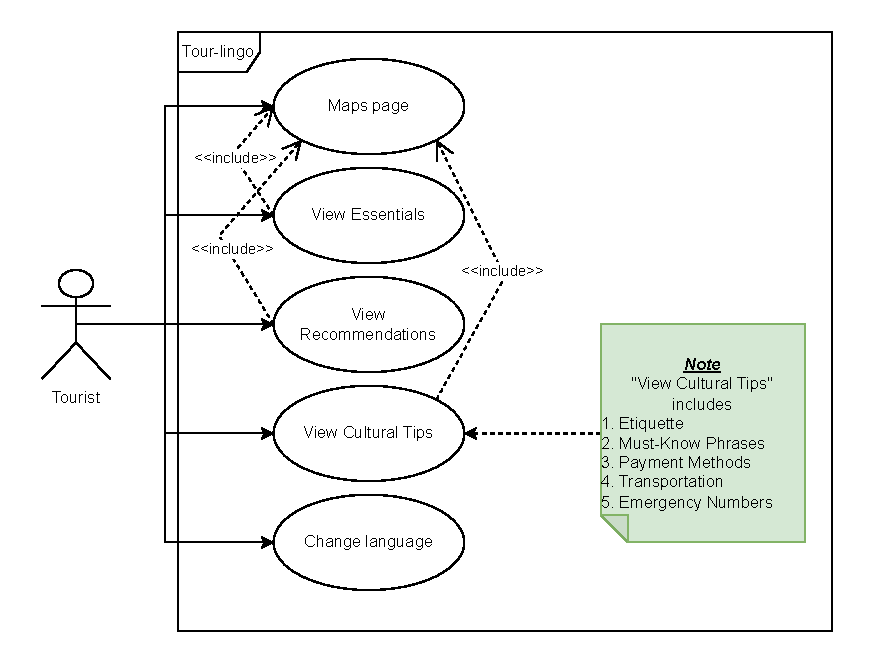
\includegraphics[width=0.5\linewidth]{chapter/05_implementation/Frontend_Usecase_Diagram.pdf}
    }
    \caption{Frontend Use Case Diagram}
    \label{fig:frontend_usecase}
\end{figure}

\import{chapter/05_implementation/integration}{ApiAndIntegration.tex}

\import{chapter/05_implementation/DeploymentResearchResults}{Deployment.tex}
\section{DON'T REVIEW THIS YET, I NEED TO GO THROUGH IT AGAIN TO SEE IF IT IS GOOD ENOUGH TO ASK FOR COMMENTS}